\section{Realisierung}

In diesem Kapitel wird die konkrete Umsetzung der Anforderungen in GWT beschreiben.
Zuerst wird die Architektur der Anwendung festgelegt. Anschließend werden konkrete
Implentierungsdetails erläutert, welche die Erstellung eigener Widgets in GWT und
mittels JSNI, das Styling in GSS sowie die Lokalisierung umfassen.

\subsection{Architektur}

Um den Anforderungen der zwei Anwendergruppen (Veranstalter und Gäste einer Party) gerecht
zu werden, entwickeln wir zwei GWT-Anwendungen. Die Admin-Oberfläche wird als Desktop-Webanwendung
entwickelt, während die Vote-App als mobile Webanwendung umgesetzt wird. Trotzdem werden
beide Anwendungen mit einer ähnlichen Softwarearchitektur implementiert.

\begin{figure}[tbh]
\centering
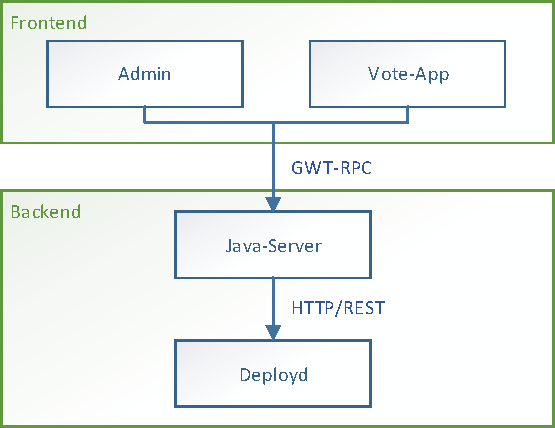
\includegraphics[width=0.7\linewidth]{Bilder/Architektur-Ueberblick}
\caption{Überblick über die Architektur der beiden Anwendungen}
\label{fig:Architektur-Ueberblick}
\end{figure}

Die Frontend-Webapplikationen kommunizieren über GWT-RPC mit einem Java-Server. Dieser dient als 
Proxy zum deployd\footnote{\url{http://deployd.com/}}-Server und enthält selbst keine Applikationslogik. Auf diese Weise umgehen wir das Problem der Same-Origin-Policy. Der deployed-Server
ist für die Persistenz der Daten und die Anwendungslogik verantwortlich und wird über eine
HTTP-Schnittstelle angesprochen.

\subsubsection{Frontend}
Innerhalb der GWT-Frontend-Anwendungen wird das MVP-Pattern zur Trennung von Steuerung und Anzeige
der Oberfläche implementiert. Der Zugriff auf das Model wird über Services ermöglicht, die intern
eine Anfrage an den Java-Server im Backend durchführen.

MVP-Architektur
- Klassendiagramm für beide (Views \& Presenter)

\subsubsection{Backend}
- Java-Server
- Als Proxy für Deployed
- Deployed zur Datenhaltung + Logik

Fabian

\subsection{Eigene Widgets}
- Search Dinge
- PlaylistEntries

Beispiele

Chris

\subsection{Styles in GSS}
Für das Styling der beiden GWT-Anwendungen verwenden wir GSS. Da es unterschiedliche Anforderungen
an Deskop- und Mobilanwendungen gibt, werden zwei Stylesheet-Dateien verwendet.

- Verknüpfung: Client-Bundle und GSS-Dateien
- Gemeinsame Styles auslagern?

Fabian

\subsection{Lokalisierung}
Beide Anwendungen sollen lokalisiert in Deutsch und Englisch angeboten werden.
Im Admin soll es möglich sein die Sprache über die Oberfläche zu ändern, während
in der Vote-App die Sprache automatisch ausgewählt wird.

Dazu verwenden wir Ressourcen-Strings (TODO).

Fabian

\subsection{JSNI}
Slider mit jQuery

Daniel